\chapter{Introduction}\label{cap:introduction}
Computational Intelligence is a research area in which nature-inspired
computational methodologies and approaches are proposed to tackle
complex real-world problems. Computational Intelligence are often used in application where the traditional methodologies are
ineffective or unfeasible. This area presents two main subareas: Fuzzy Logic
\cite{Fuzzy:Ziimermann2001}, population based techniques and artificial neural networks \cite{NN:Rumelhart1987}.

The main population based approaches are: evolutionary computation (Genetic
Algorithm (GA) \cite{GA:Mitchell1998} \cite{GA:Guo2008}, Differential Evolution
(DE) \cite{DE:Gao2010} \cite{DE:Prince2005}, Evolutionary Strategies (ES)
\cite{ES:Beyer2001a} \cite{ES:Beyer2001b}), swarm based optimization
methods (Particle Swarm Optimization (PSO) \cite{PSO:Eberhart1995}
\cite{PSO:Eberhart1995a}, Ant Colony Optimization (ACO) \cite{ACO:Dorigo1999}
\cite{ACO:Dorigo2005}, Artificial Bee Colony (ABC) \cite{ABC:Karaboga2005}
\cite{ABC:Karaboga2006}, Fish School Search (FSS) \cite{FSS:Bastos-Filho2008},
Fish Swarm Algorithm (FSA) \cite{FSA:Yazdani2012}, Bacterial Foraging Algorithm
(BFA) \cite{BFA:Muller2002}, Bacterial Foraging Optimization (BFO)
\cite{BFO:Das2009}, Glowworm Swarm Optimization (GSO)
\cite{GSO:Krishnanand2009}, Firefly Algorithm (FA) \cite{FA:Yang2009}), among
others.

Swarm intelligence became one branch of the computational intelligence which experienced a huge expansion in recent years. The expression
`Swarm Intelligence' was introduced by Gerardo Beni and Jing Wang
in 1989 \cite{SI:Beni1989}. The term `swarm' is used basically to refer any
structured collection of agents able to interact. The swarm intelligence systems
are composed by agents that interact among each other and their environment. From this
interaction, global behaviors that can not observed in the agents
individually, emerge.

The swarm Intelligence techniques were originated from the study of collective
behavior of microorganisms, animals and insects in the nature. They are
commonly used to solve optimization and search problems. These algorithms are
self-organized, distributed, autonomous, flexible and dynamic.

The main properties of a swarm intelligence system are \cite{SI:Serapiao2009}:
\emph{proximity} - the agents should be able to interact; \emph{quality} - the
agents should be able to evaluate their behaviors; \emph{diversity} - allows
the system to react to unexpected situations; \emph{stability} - not every
environment variations should affect the behavior of an agent;
\emph{adaptability} - adequacy to environment variations capability.

Among several approaches, some of them are used to tackle continuous problems without
constraints. We can cite some of them: PSO, ABC and FSS.

The PSO algorithm was inspired in the behavior of bird flocks (observe Figure
\ref{fig:flock_birds}). Basically, there is a swarm of particles, where
each particle is a potential solution of the problem. The particle moves through the search space by updating its velocity and position. The velocity is calculated
considering the best position found by the individual (cognitive memory) and the
best position found by its neighborhood (social memory).
\begin{figure}[!h]
\centering
 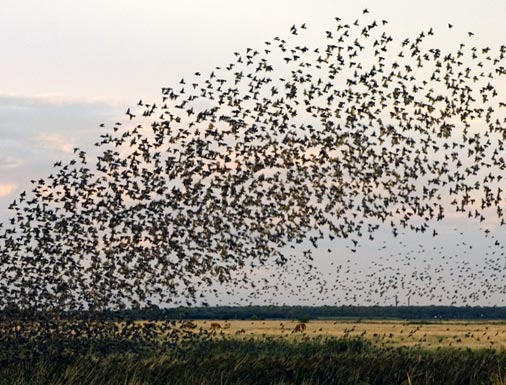
\includegraphics[width=0.45\textwidth]{image/flock_of_birds.jpg}
 \caption{\small{Example of a bird flock in the nature (Adapted from:
\cite{SI:Bird2012}).}}
 \label{fig:flock_birds}
\end{figure}

The ABC algorithm was inspired in the behavior of honey bees (observe Figure
\ref{fig:bee_colony}). In this algorithm, the bee colony has three type of bees:
employed bees, onlookers and scouts. The food sources are the potential solutions of
the problem. Each food source has an associated employed bee. The
employed bees explore the food source and share the information (through the
dance of the bees) to the onlooker bee. These bees are responsible to choose a
food source (preferentially, the richer one) and explore it. When the employed
bee abandons the food source, it becomes a scout bee and, then, will seek a
new food source.
\begin{figure}[!h]
\centering
 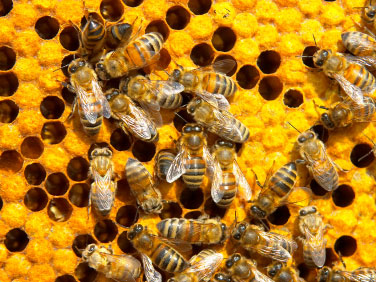
\includegraphics[width=0.45\textwidth]{image/bee_colony.png}
 \caption{\small{Example of bee colony in the nature (Adapted from: \cite{SI:Bee2012}).}}
 \label{fig:bee_colony}
\end{figure}

The FSS algorithm was inspired in the behavior of school of fish (observe Figure
\ref{fig:school_fish}). In this algorithm, the position of the fish is a
potential solution of the problem. Their weights represent the success during
the search process. The execution of the algorithm is based on the
operators that were inspired in the individual and collective behavior of fish
in order to guarantee the survivability of the entire group. As a consequence, the fish move to the most promising food source. The fish school
will direct the sense of its search based on the increasement of the weight of
the fish. Depending of the granularity of the search, the swarm can expand or
contract.
\begin{figure}[!h]
\centering
 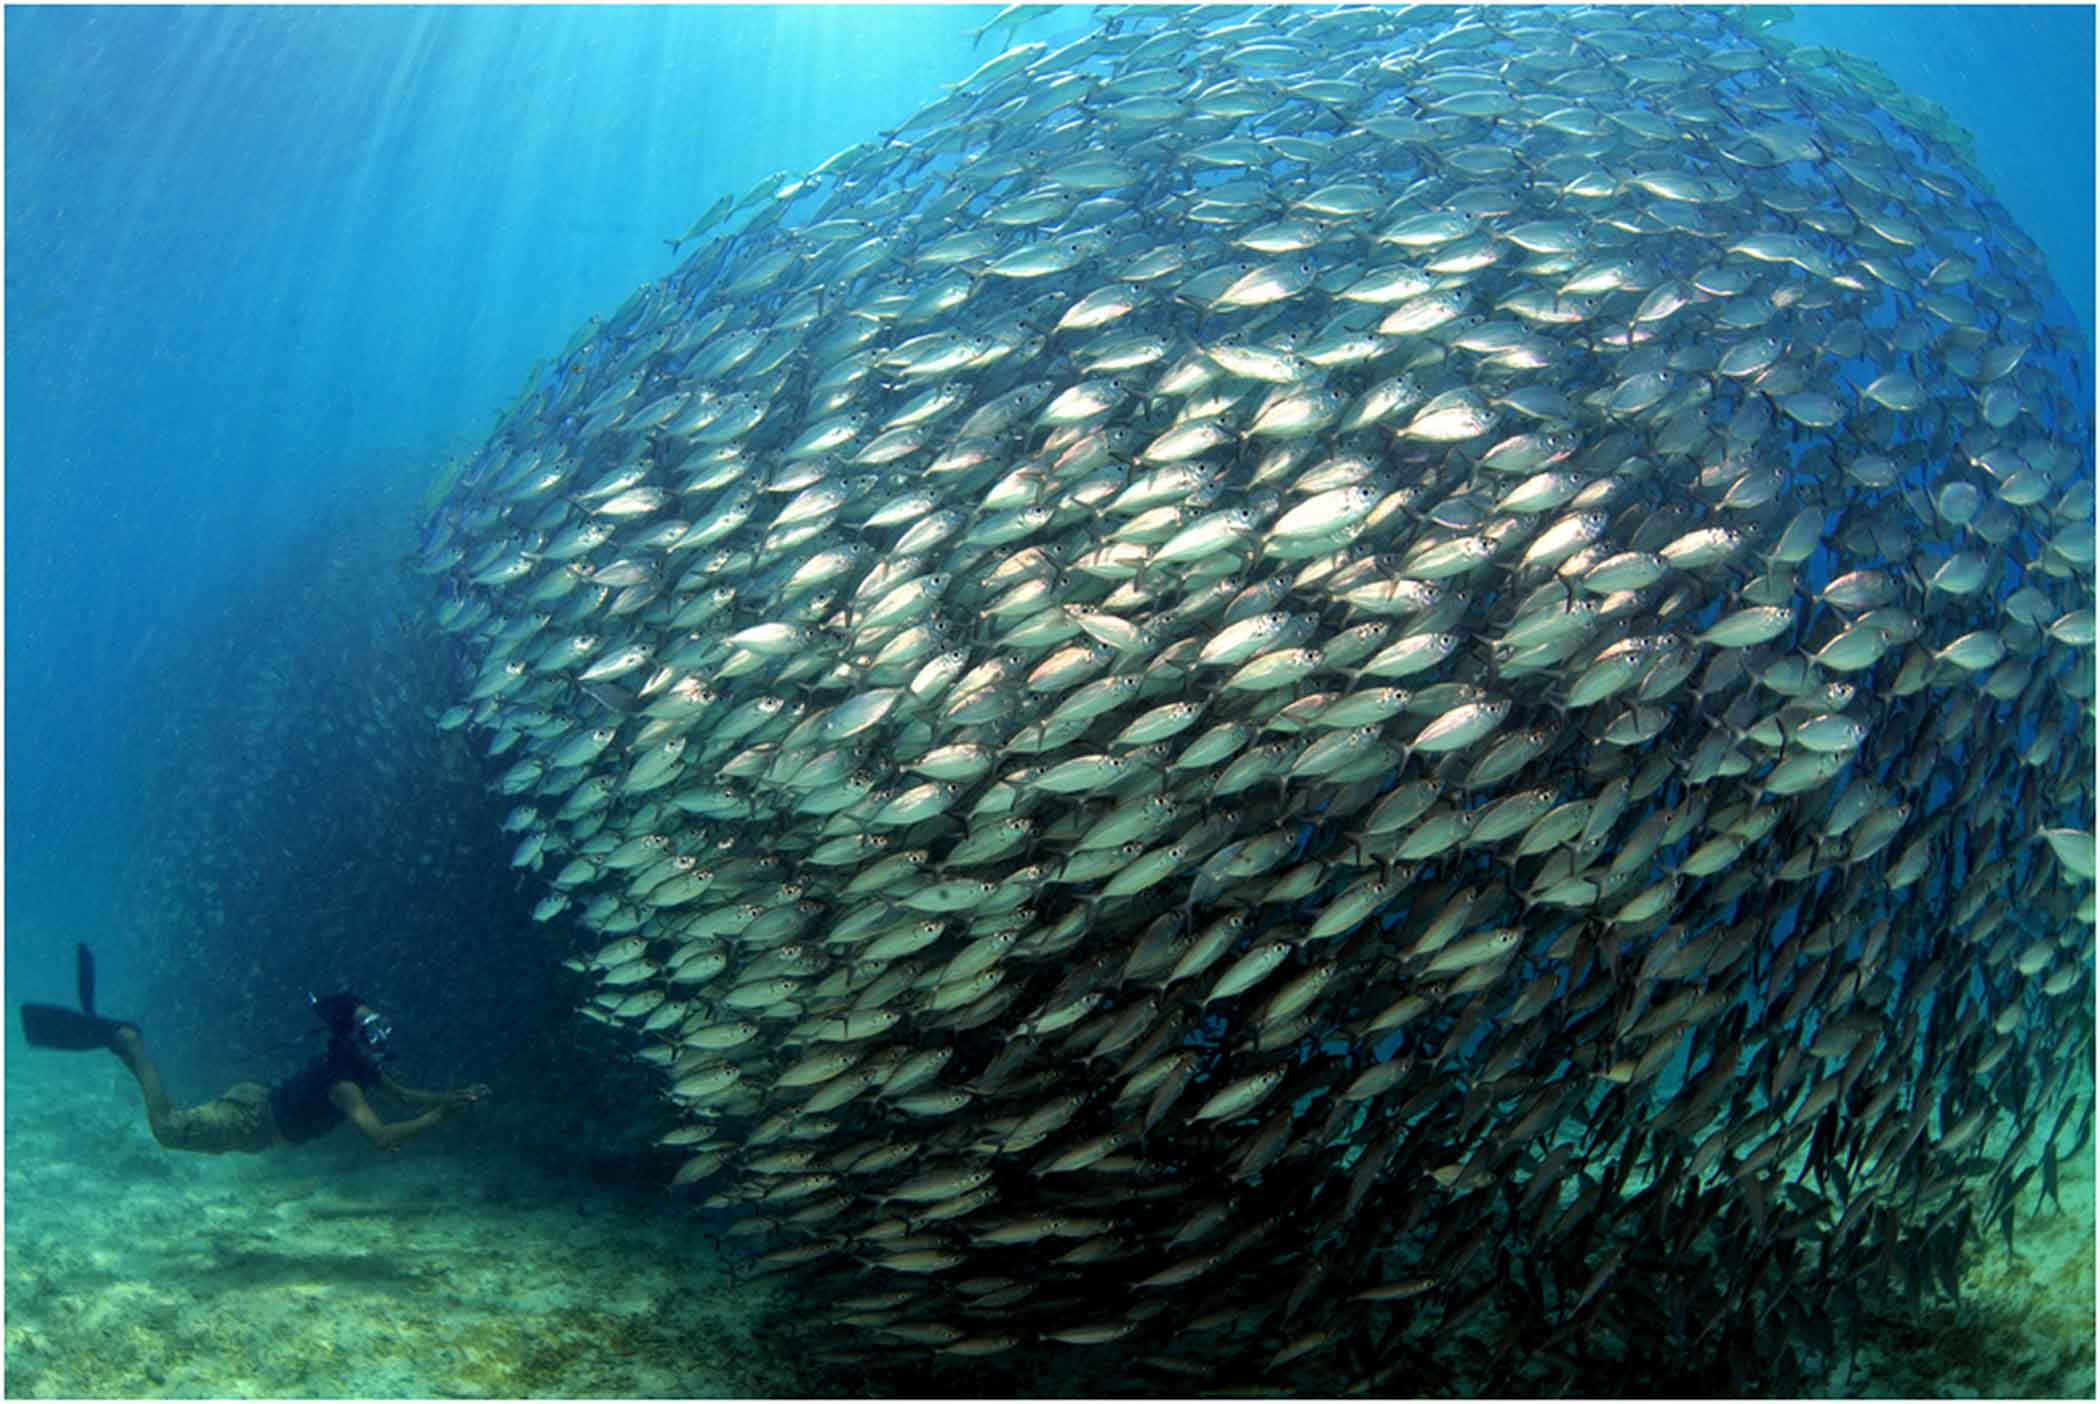
\includegraphics[width=0.45\textwidth]{image/school_of_fish.jpg}
 \caption{\small{Example of a fish school in the nature (Adapted from:
\cite{SI:Fish2012}).}}
 \label{fig:school_fish}
\end{figure}

Each one of these algorithms has particularities, strengths and weaknesses.
Moreover, they have mechanisms to simultaneously represent success, to guarantee
convergence and maintain diversity. It is important to emphasize that these
algorithms do not have mutually exclusive characteristics. For example, the PSO
algorithm has a good convergence mechanism, but it does not have the capability
to maintain the diversity of the swarm. On the other hand, the ABC algorithm has
a satisfactory ability to generate diversity. Thus, we believe it is possible to combine these algorithms to provide both features.

\section{Motivation and Objectives}
The optimization problems present several challenges, such as: the ``Curse of Dimensionality'' effect \cite{SI:Houle2010} \cite{SI:Powell2007} \cite{SI:Radovanovic2010} and the ``No Free Lunch'' theorem \cite{SI:Wolpert1995} \cite{SI:Wolpert1997} \cite{SI:Droste2002}.

The curse of dimensionality refers to the phenomenon that arises when analyzing
high-dimensionality search spaces (often with hundreds or thousands of
dimensions). This phenomenon generally does not occur in low-dimensionality.
This means that the volume of the search space increases when the
dimensionality increases. In this scenario, it is expected that some optimization algorithms work well to solve
problems with low dimensionality, but they can present a poor performance and high computational cost as the number of dimensions increase.

The theorem \emph{No Free Lunch} was introduced by David Wolpert and William G.
Macready \cite{SI:Wolpert1995}. This theorem states that if an optimization
algorithm achieves better results in some classes of problems, it must present worse
results in other ones. Thus, it is important to define which group of
problems an optimization algorithm can tackle. In principle, there is not a single
optimization algorithm that is able to solve all types of problems with the best possible performance.

The swarm intelligence algorithms have the ability to solve complex problems.
Many of them have their performance mitigated when they are applied to very complex problems. Scenarios with high
dimensionality, continuous variables, multimodal search spaces and variables with different degrees of
dependency allows one to simulate optimization problems with characteristics that are similar to the ones presented in the real world.

In this scenario, combining swarm intelligence algorithms can be an
alternative to solve complex problems with high dimensionality. Therefore, the main objective is to study the swarm intelligence approaches in order
to find the main characteristics of them, indicating possible combinations so
the limitations of the algorithms can be mitigated. Finally, the combined
approach must be applicable to handle optimization problems with high-dimensionality.

This dissertation proposes to combine the Adaptive Particle Swarm Optimization (APSO) algorithm with the ABC algorithm. The APSO algorithm has the adaptive behavior that guarantees the convergence ability. The Artificial Bee Colony (ABC) algorithm has the diversity capability. Considering these characteristics, the proposal is to develop an operator based on artificial bees to generate diversity in order to be included it in the APSO algorithm.

\section{Contributions}
The main contribution of this dissertation is the combined algorithm called Adaptive Bee and Particle Swarm Optimization (ABeePSO). This algorithm is a proper combination of two well known swarm intelligence algorithms: Adaptive Particle Swarm Optimization (APSO) \cite{APSO:Zhan2009} and Artificial Bee Colony (ABC) \cite{ABC:Karaboga2005}. The proposed algorithm has an new operator of maintain the diversity in the swarm. The proposal combines the peculiar behavior of the guide bees of the ABC algorithm and uses the centroid concept to spread the swarm, which is based on the concept proposed in the FSS algorithm. The results show that our proposal achieved better results in complex functions with high-dimensional search spaces. This means that our proposal can maintain good convergence and has the capability to escape from local minima when the search space has a high number of dimensions, mainly in multimodal functions.


\section{Document Structure}
For a better understanding of this dissertation, we indicate a sequential reading. The rest of the dissertation is organized as follows:
\begin{itemize}
  \item Chapter \ref{cap:introduction} presented the motivation and the objectives of this dissertation;
  \item Chapter \ref{cap:Swarm} describes the state-of-art regarding swarm intelligence optimizers;
  \item Chapter \ref{cap:contribution} describes our proposal, the ABeePSO algorithm;
  \item Chapter 4 presents the methodology and the simulation setup;
  \item Chapter 5 presents the results;
  \item Chapter 6 describes presents some conclusions and future works;
  \item Appendix A presents the publications of the research.
\end{itemize}


